%%%%%%%%%%%%%%%%%%%%%%%%%%%%%%%%%%%%%%%%%%%%%%
% Power Rules: Practical Advice for Computing Statistical Power
% Preprint of the article in Political Analysis: the main text. The appendices are
% in power-rules-appendix.tex; bibliography.bib and Figure 1 (geometry.pdf) are beside it.
% The scripts that make the HTML version (html-version/, kept out of this repository)
% copy the title, the abstract (between the lines "%%% begin abstract" and
% "%%% end abstract"), and the body (between "%%% begin body" and "%%% end body")
% out of this file, so keep those lines.
%%%%%%%%%%%%%%%%%%%%%%%%%%%%%%%%%%%%%%%%%%%%%%
\documentclass[12pt]{article}

% Page and fonts
\usepackage{fullpage}
\usepackage{setspace}
\usepackage[T1]{fontenc}
\usepackage{lmodern} % Latin Modern: Computer Modern, as in the earlier preprint, with T1 accents
\usepackage[nopatch]{microtype}
\usepackage[table]{xcolor}
\usepackage{graphicx}
\usepackage[labelsep=period,font=small]{caption} % "Table 1." as in the PA class

% Packages the manuscript loads (as in the PA preamble)
\usepackage{booktabs}
\usepackage{array}
\usepackage{mathtools} % loads amsmath; provides \mathclap
\usepackage{amsfonts}
\usepackage{amssymb}
\usepackage{textcomp} % for \textrightarrow
\usepackage{tabularx}
\usepackage{lscape} % For landscape orientation
\usepackage{multirow} % For multirow cells

% Citations and references: the same style and options as the PA class
\usepackage[authordate-trad,noibid,backend=biber,natbib,footmarkoff]{biblatex-chicago}
\addbibresource{bibliography.bib}

\newcommand{\titlemain}{Power Rules}
\newcommand{\titlesub}{Practical Advice for Computing Statistical Power}
\usepackage{hyperref}
\usepackage{xurl} % long URLs break anywhere, rather than stretch the spaces in the line
\hypersetup{
  pdftitle={\titlemain: \titlesub},
  pdfauthor={Carlisle Rainey},
  colorlinks,
  linkcolor=black,
  citecolor=black,
  urlcolor=blue!50!black
}

% Headings, as in the earlier preprint
\usepackage{titlesec}
\titleformat{\section}
 {\normalfont\sffamily\Large\bfseries}
 {\thesection}{1em}{}
\titleformat{\subsection}
 {\normalfont\sffamily\bfseries}
 {\thesubsection}{1em}{}
\titleformat{\paragraph}[runin]
 {\normalfont\sffamily\bfseries}
 {}{0pt}{}

% Appendix sections print as "Appendix 1", as in the PA class
\makeatletter
\renewcommand\appendix{\par
  \setcounter{section}{0}%
  \setcounter{subsection}{0}%
  \gdef\thesection{Appendix \@arabic\c@section}%
  \titleformat{\section}{\normalfont\sffamily\Large\bfseries}{\thesection.}{1em}{}%
}
\makeatother

% Floats: the manuscript places its tables with [h] or [ht], which a double-spaced page often
% cannot honor, and LaTeX then holds them to the end; allow a page of floats instead
\let\origtable\table
\let\endorigtable\endtable
\renewenvironment{table}[1][]{\origtable[htbp]}{\endorigtable}
\renewcommand{\topfraction}{0.85}
\renewcommand{\textfraction}{0.1}
\renewcommand{\floatpagefraction}{0.75}

% The blanks (\underline{~~~~~} in the manuscript) at the width the PA build prints them,
% 1.3 times the type size (five spaces would be wider in this font); other underlines unchanged
\makeatletter
\NewCommandCopy{\pr@underline}{\underline}
\def\pr@blank{~~~~~}
\DeclareRobustCommand{\underline}[1]{\def\pr@arg{#1}%
  \ifx\pr@arg\pr@blank\pr@underline{\hbox to 1.3\dimexpr\f@size pt\relax{}}\else\pr@underline{#1}\fi}
\makeatother

% Table header rows (\headrow in the PA class): no gray fill, since the tables here are in the
% booktabs style
\newcommand{\headrow}{}

% Theorem/rule environment (as in the PA preamble)
\usepackage{mdframed}
\usepackage{amsthm}
\usepackage{thmtools}
\usepackage{thm-restate}

\declaretheoremstyle[
  headfont=\normalfont\bfseries,
  bodyfont=\normalfont,
  notefont=\normalfont\bfseries,
  postheadspace=0.5em,
  headpunct={:},
  spacebelow=\medskipamount,
  spaceabove=\medskipamount,
  mdframed={
    nobreak=true,
    linecolor=gray!20,
    backgroundcolor=gray!10,
    linewidth=0.5pt,
    roundcorner=5pt,
    innertopmargin=5pt,
    innerbottommargin=5pt,
    innerrightmargin=5pt,
    innerleftmargin=5pt
  }
]{mytheoremstyle}
\declaretheorem[name=Rule, style=mytheoremstyle]{rule0}

% Lists (as in the PA class and preamble)
\usepackage{enumitem}
\renewcommand{\theenumi}{\arabic{enumi}.}
\renewcommand{\labelenumi}{\theenumi}
\renewcommand{\theenumii}{\alph{enumii}.}
\renewcommand{\labelenumii}{\theenumii}
\renewcommand{\theenumiii}{\roman{enumiii}.}
\renewcommand{\labelenumiii}{\theenumiii}
\renewcommand{\theenumiv}{\Alph{enumiv}.}
\renewcommand{\labelenumiv}{\theenumiv}
\setlist{noitemsep,leftmargin=\parindent}
\setlist{nolistsep}

\long\def\symbolfootnote[#1]#2{\begingroup%
\def\thefootnote{\fnsymbol{footnote}}\footnote[#1]{#2}\endgroup}

\begin{document}

\begin{center}
{\huge \textbf{\titlemain}}

\vspace{0.4cm}

{\Large\textbf{\titlesub}}

\vspace{1cm}

Carlisle Rainey\symbolfootnote[2]{Carlisle Rainey is Professor of Political Science, Florida State University, 540 Bellamy, Tallahassee, FL, 32306. (\href{mailto:crainey@fsu.edu}{crainey@fsu.edu}).}

\vspace{1cm}
\today
\vspace{5mm}

Latest version \href{https://osf.io/preprints/osf/5am9q}{here}.
\end{center}

\vspace{5mm}

{\centerline{\textbf{Abstract}}}
\begin{quote}\noindent
%%% begin abstract
Recent work emphasizes the importance of statistical power in the social sciences and shows that power tends to be very low.
In this paper, I offer simple rules to compute power for balanced, between-subjects designs.
For balanced, between-subjects designs (e.g., common for survey experiments), these rules are sufficient for a complete, compact, and compelling power analysis for treatment effects and interactions.
Most importantly, these rules help researchers develop a sharp intuition about statistical power, lower the barrier to entry for researchers new to thinking carefully about statistical power, and help researchers design powerful, informative experiments.
%%% end abstract
\end{quote}

\thispagestyle{empty}
\newpage

\doublespace
\setcounter{page}{1}

%%% begin body

\section*{Introduction}

Experiments continue to grow in political science \citep{Druckman2021}, and designing an experiment requires us to either select an appropriate sample size or evaluate whether a given sample size is sufficient for our goals.\footnote{
  For example, the \emph{Journal of Politics} guidelines for registered reports note that ``a detailed justification of the proposed sample size is crucial'' (accessed October~20, 2026; \href{https://web.archive.org/web/20250702024222/https://www.journals.uchicago.edu/journals/jop/registered-report-guidelines}{persistent link}).
  The \emph{Journal of Experimental Political Science} requires authors to ``explain how the sample size was determined and note statistical power'' (accessed October~20, 2026; \href{https://web.archive.org/web/20261020192159/https://www.cambridge.org/core/journals/journal-of-experimental-political-science/information/author-instructions/preparing-your-materials}{persistent link}).
  Time-sharing Experiments for the Social Sciences (TESS) notes that power analysis is ``encouraged'' (accessed October~20, 2026; \href{https://web.archive.org/web/20261020192157/https://www.tessexperiments.org/info/howtosubmit}{persistent link}).
  The National Institutes of Health (NIH) provides several examples to ``demonstrate rigor,'' and all examples include a discussion of statistical power (accessed October~20, 2026; \href{https://web.archive.org/web/20261020192244/https://grants.nih.gov/policy-and-compliance/policy-topics/reproducibility/resources}{persistent link}).
  The popular OSF pre-registration template includes a field for a sample size rationale, which could include a power analysis \citep{Bowman2020}.}
Statistical power, or the chance of rejecting the null hypothesis for a given treatment effect, is a common, powerful way to select or evaluate a sample size.
The consequences of low power are increasingly understood: low power can lead to wildly overestimated treatment effects \citep{Gelman2014} and ambiguous results that are difficult to publish (e.g., \citealt{Alrababah2023}).
Nonetheless, \citet{ArelBundock2022} argue that only about 10\% of statistical tests in political science have at least 80\% power to detect the consensus effect in their literature.
\citet{Stommes2023} find that regression discontinuity studies in political science tend to be underpowered as well.
And political science is hardly unusual \citep{Cohen1962, Button2013, Ioannidis2017, Stanley2018, Yang2023}.
Underscoring their important findings, \citet[44--45]{ArelBundock2022} emphasize: ``our research community must address the problems of low power and selection on significance with institutional, methodological, and theoretical remedies.''

One apparent problem is that while political scientists understand estimation and inference for experimental data very well (e.g., least squares regression with robust standard errors), political scientists are less comfortable thinking about statistical power prior to data collection.
This apparent discomfort is not without reason.
Power analysis requires specialized software or tedious simulation.
Most specialized software, such as G*Power \citep{Faul2007, Faul2009}, follows the conventions of psychology.
The language (e.g., Cohen's \emph{d}) and style of analysis (e.g., ANCOVA) can make the software awkward for political scientists to use, though these obstacles are of course not insurmountable.\footnote{
  For example, the power resources that the \emph{Journal of Politics} provides include links to several resources for planning sample size in experiments, but many of these resources are directed primarily at psychologists.
  }
Most importantly, political scientists tend to focus on treatment effects on the scale of the outcome (e.g., \citealt{King2000}), while psychologists are more comfortable with standardized effect sizes.\footnote{
  \citet{Lakens2022} offers a careful and thorough discussion of sample size justifications for an audience of psychologists, but (appropriately) uses terms common in psychology.
  For example, Lakens centers much of his discussion around Cohen's \emph{d}, a standardized effect size used often in psychology but less often in political science.
  }
And while psychologists rely on a range of procedures to test hypotheses, political scientists typically use least squares regression with robust standard errors.
In political science, recent conceptual work and statistical software \citep{Blair2019, Blair2023} make complex simulations to comprehensively evaluate research designs more accessible, but simulation to obtain statistical power remains challenging compared to analyzing experimental data.
Political scientists lack a gateway between the simple, robust tools of inference using experimental data and the complex, tedious tools that allow complete and careful evaluations of research designs.
This paper can help create the link by offering useful approximations for balanced, between-subjects designs or by helping build intuition that transfers to more complex designs.

In this paper, I offer several simple rules for assessing the statistical power of a balanced, between-subjects design (i.e., a design that assigns an equal number of subjects to each experimental condition).
For these balanced, between-subjects designs (e.g., common for survey experiments), the rules are sufficient to demonstrate adequate power for treatment effects and interactions.
I tightly connect the rules for statistical power to the logic of estimation and inference for experimental data in political science (least squares regression, robust standard errors, and confidence intervals).
There is tremendous value in simple, conceptual rules of thumb---the kind of rules that allow us to predict the statistical power of an experiment with paper, a pencil, and (perhaps) a pocket calculator. %\footnote{
%  Paper-and-pencil calculations are valuable, for two reasons.
%  First, predicting statistical power involves some guesswork.
%  Specialized software and simulations bring an air of exactness that does not match the spirit of the task.
%  With paper-and-pencil calculations, it seems easier to remember that task is to make an informed guess using clear assumptions.
%  Second, paper-and-pencil work constantly reminds us how inputs relate to outputs.
%  Since we are \emph{designing} experiments and have freedom to make different design choices, it can be helpful to be constantly reminded of the relationship between inputs and outputs.
%  }
While specialized software and complex simulations are helpful (and essential in some cases), simple rules have several benefits:
(1) simple rules can make statistical power accessible, rather than seem like a mystical quantity;
(2) simple rules allow us to reason fluently about design choices;
(3) simple rules can reduce the chance of making big errors by giving us a ballpark starting point even if we ultimately rely on a more sophisticated approach; and
(4) for balanced, between-subjects designs, simple rules are sufficient to justify a sample size, and simulations and specialized software are unnecessary.
I explain the intuition of each rule, describe how we can use the rule to plan or evaluate a study, and give examples.
Appendix~4 collects all seven rules in one place for quick reference.

Before turning to the rules, I should clearly delineate the type of experiments they cover, so that a reader can gauge whether the rules apply to their design.
The rules in the main text apply to balanced (i.e., treatment and control groups are the same size), between-subjects experiments with independent assignment.
I assume that we estimate the treatment effect with least squares regression and robust standard errors, and that we test a directional hypothesis about that effect.
A researcher whose experiment fits this description can apply the rules in the main text directly.\footnote{
  This includes experiments that analyze a multi-item index rather than a single item. A researcher analyzing an index can treat the index itself as the outcome (e.g., let $\widetilde{SD(Y)}$ in Rule~\ref{rule:sd-to-se} be the standard deviation of the index rather than of a single item) and then proceed through the remaining rules as usual.
  }
For researchers whose experiment does not fit this description, we can accommodate several common complications discussed in Appendices~1 and~2.
Appendix~1 gives the factors for power levels other than 80\% or 95\% for both the one-sided and two-sided conventions.
Appendix~2 adapts the rules to unbalanced assignment, clustered assignment, blocked random assignment, and interactions.
For designs with other complications, the rules might still provide a ballpark starting point, but a careful power analysis requires simulation or specialized software.

\section*{Review: The Estimation and Inference Framework}

Throughout this discussion, I assume that we use ordinary least squares and robust standard errors to estimate the treatment effect.
I assume size-0.05, one-sided tests of directional hypotheses (i.e., tests at the 0.05 significance level, or $\alpha = 0.05$) evaluated in practice using 90\% confidence intervals.
The one-sided test is a natural default because we test a directional hypothesis.
Some researchers instead prefer two-sided tests, which are equivalent to 95\% confidence intervals.
I report the factors for two-sided tests alongside the one-sided factors throughout, so that researchers can apply the rules under either convention.
To make the discussion more natural, I borrow the language of survey experiments and describe the experimental units as ``respondents,'' but the logic generalizes to other types of units (e.g., villages).

Formally, I assume potential outcomes $\mathcal{Y}_{i}(1)$ if assigned to treatment and $\mathcal{Y}_{i}(0)$ if assigned to control for respondent $i$ of $N$.
An experiment might use more than two conditions, but for the sake of the discussion below, I focus on the statistical power of a comparison of just \emph{two} of these conditions, which I call treatment and control.\footnote{
   In many experiments, there will be multiple comparisons of interest.
   In this case, we need to compute the statistical power for each test separately.
   As the \textit{Journal of Politics} guidelines note: ``Power calculations should be performed for each test individually'' (accessed October~20, 2026; \href{https://web.archive.org/web/20250702024222/https://www.journals.uchicago.edu/journals/jop/registered-report-guidelines}{persistent link}).
  }
For these two conditions, we want to make inferences about the average treatment effect $\tau = \frac{1}{N}\sum_{i = 1}^{N}{\mathcal{Y}_{i}(1)} - \frac{1}{N}\sum_{i = 1}^{N}{\mathcal{Y}_{i}(0)}$ (which I refer to as a ``treatment effect'' throughout).

To make inferences about $\tau$, we randomly assign $n_{1}$ respondents to treatment and $n_{0}$ respondents to control, where $N = n_{1} + n_{0}$.\footnote{
  Note that $N$ represents the \emph{total number of respondents} in the comparison, while $n_{d}$ represents the number of respondents \emph{in condition} $d \in \{0, 1\}$.
  Below, I assume equal numbers of respondents in each condition, so I let $n$ represent the number of respondents per condition, which is a convenient quantity when thinking about experimental design and statistical power.
  }
We create an indicator variable $D_{i}$ that equals 1 if the respondent is assigned to treatment and 0 if the respondent is assigned to control.
Then we create the observed outcome $Y_{i} = \mathcal{Y}_{i}\left( D_{i} \right)$ by assigning $Y_{i}$ the potential outcome under treatment if $D_{i} = 1$ and the potential outcome under control if $D_{i} = 0$.
Then we estimate the treatment effect using $\widehat{\tau} = \frac{1}{n_{1}}\sum_{i = 1}^{N}{D_{i} \cdot Y_{i}} - \frac{1}{n_{0}}\sum_{i = 1}^{N}{\left( 1 - D_{i} \right) \cdot Y_{i}}$, which we compute in practice using least squares estimates of the model $Y_{i} = \alpha + \tau \cdot D_{i} + \epsilon_{i}$.
In some cases, we might increase the precision of the estimates by including variables measured pre-treatment as control variables in the regression model.

To estimate the standard error of $\widehat{\tau}$, we use Neyman's ([1923] \citeyear{Neyman1923}) conservative variance estimator.\footnote{
  Specifically, $\widehat{Var}\left( \widehat{\tau} \right) = \frac{s_{1}^{2}}{n_{1}} + \frac{s_{0}^{2}}{n_{0}}$, where $s_{1}^{2}$ and $s_{0}^{2}$ represent the sample variances in the treatment and control groups, respectively, and ${\widehat{SE}}_{\widehat{\tau}} = \sqrt{\widehat{Var}\left( \widehat{\tau} \right)}$.
  }
In practice, we use an HC2 heteroskedasticity-robust variance estimator (or a closely related variant).\footnote{
  \citet[367--368]{Samii2012} show that the HC2 estimator is equivalent to Neyman's estimator. For testing, \citet[1764--1765]{Li2017} provide several additional (seemingly innocuous) regularity conditions such that a finite-population central limit theorem holds and $\left\lbrack \widehat{\tau} - \Phi_{std}^{-1}\left( 1 - \alpha \right) \cdot {\widehat{SE}}_{\widehat{\tau}},\widehat{\tau} + \Phi_{std}^{-1}\left( 1 - \alpha \right) \cdot {\widehat{SE}}_{\widehat{\tau}} \right\rbrack$ is an asymptotically conservative $\left( 1 - 2\alpha \right) \cdot 100\%$ confidence interval, where $\Phi_{std}^{-1}$ is the inverse of the standard normal CDF.
  }
We can use the 90\% confidence interval $\left\lbrack \widehat{\tau} - 1.64 \cdot {\widehat{SE}}_{\widehat{\tau}},\widehat{\tau} + 1.64 \cdot {\widehat{SE}}_{\widehat{\tau}} \right\rbrack$ to conduct size-0.05 tests of directional hypotheses by rejecting a null hypothesis if and only if \emph{all} values in the 90\% confidence interval are consistent with the research hypothesis \citep{Rainey2014, McCaskey2015}.
A researcher using a size-0.05, two-sided test instead rejects the null hypothesis when the 95\% confidence interval excludes zero.
For the 95\% confidence interval, the 1.64 threshold becomes 1.96 so that the 95\% confidence interval is $\left\lbrack \widehat{\tau} - 1.96 \cdot {\widehat{SE}}_{\widehat{\tau}},\widehat{\tau} + 1.96 \cdot {\widehat{SE}}_{\widehat{\tau}} \right\rbrack$.

\section*{Rules~\ref{rule:power-int} and~\ref{rule:power-z}: What Is Statistical Power?}

In a designed experiment, we usually have a theoretically motivated research hypothesis that we would like to test.
This research hypothesis implies a null hypothesis that we hope to reject.
For simplicity, I assume throughout much of this paper that we hypothesize a \emph{positive} treatment effect so that $H_{R}:\tau > 0$.
The extension to a negative treatment effect is obvious.

Imagine that we repeatedly re-randomize to treatment and control and compute $\widehat{\tau}$ for each repetition.
Then $\widehat{\tau}$ will vary across these repeated experiments.
We refer to the distribution of $\widehat{\tau}$ across these hypothetical
repeated experiments as the \emph{sampling distribution} of $\widehat{\tau}$.
This sampling distribution is typically centered over the treatment effect (i.e., $\widehat{\tau}$ is unbiased or nearly so).
Importantly, the standard deviation of the sampling distribution of $\widehat{\tau}$ is called the \emph{standard error}, and ${\widehat{SE}}_{\widehat{\tau}}$ is usually a precise estimator of the standard error.

If the research hypothesis $H_{R}:\tau > 0$ is correct, then the sampling distribution of $\widehat{\tau}$ lies mostly to the right of zero.
However, we will only claim that $\tau > 0$ if the entire 90\% confidence interval is larger than zero, or, equivalently, if $\widehat{\tau} - 1.64 \cdot {\widehat{SE}}_{\widehat{\tau}} > 0$.
This means that we must design our experiment so that the sampling distribution falls relatively far from zero.

We say that the statistical \emph{power} of an experiment is the chance of rejecting the null hypothesis \emph{for a particular treatment effect} $\tau$.
For example, we say that an experiment has ``80\% power to detect a treatment effect of \underline{~~~~~}'' if
$\widehat{\tau} - 1.64 \cdot {\widehat{SE}}_{\widehat{\tau}} > 0$ in 80\% of repeated experiments.
Similarly, we say that the experiment has ``95\% power to detect a treatment effect of \underline{~~~~~}'' if $\widehat{\tau} - 1.64 \cdot {\widehat{SE}}_{\widehat{\tau}} > 0$ in 95\% of repeated experiments.
By convention, 80\% power is the minimal standard for ``adequate'' statistical power \citep[56]{Cohen1988}, but others recommend higher power, such as 95\%.\footnote{
  For example, the \textit{Journal of Politics} recommends ``a power of at least 0.90, ideally 0.95, to detect anticipated/relevant effect sizes'' for registered reports (accessed October~20, 2026; \href{https://web.archive.org/web/20250702024222/https://www.journals.uchicago.edu/journals/jop/registered-report-guidelines}{persistent link}).
  \textit{Nature Human Behaviour} requires that ``the a priori power must be 0.95 or higher for all proposed hypothesis tests'' for registered reports (accessed October~20, 2026; \href{https://web.archive.org/web/20261020192546/https://www.nature.com/nathumbehav/submission-guidelines/registeredreports}{persistent link}).
  }

It turns out that statistical power is determined by the treatment effect and the
standard error of the estimate.
To compute the statistical power of an experiment, we must make assumptions or ``informed guesses'' about certain quantities.
I denote these assumed values with a tilde. For example, I denote the assumed treatment effect as $\widetilde{\tau}$.\footnote{
  I use three different $\tau$s: the \emph{actual} treatment effect $\tau$, the treatment effect \emph{assumed for the sake of computing power} $\widetilde{\tau}$, and the \emph{estimated} treatment effect $\widehat{\tau}$.
  I read the tilde notation as ``assumed to compute power.''
  For example, I read $\widetilde{\tau}$ as ``the treatment effect assumed
  to compute power.''
  The tilde notation also means ``Wait! Think about this carefully; it is an assumption requiring judgment.''}
This just means ``the treatment effect we are assuming for the sake of computing statistical power.''

How can we compute the statistical power of an experiment?
An intuitive approach uses the construction of the 90\% confidence interval.
Recall that we will reject the null hypothesis if the lower bound of the 90\% confidence interval falls above zero.
The arms of the 90\% confidence interval are about 1.64 standard errors wide.\footnote{
  I write ``about'' 1.64 standard errors because in practice we use the \emph{estimated} standard error, not the actual standard error.
  However, the estimated standard error is sufficiently precise to treat
  the two interchangeably in this context.
  }
This means that we will reject the null hypothesis if the estimate of the treatment effect is larger than 1.64 standard errors.
Thus, the power of the study is the percent of the sampling distribution that is larger than 1.64 standard errors.
Recall that the sampling distribution is approximately normally distributed and centered over the treatment effect $\tau$ with standard deviation equal to the standard error of the estimate of $\tau$.\footnote{
  Rule~\ref{rule:power-int} is exact when (a) $\widehat{\tau}$ is exactly normally distributed with mean $\tau$ and standard deviation $SE$ and (b) $SE$ is known rather than estimated. Condition (a) holds in finite samples when errors are exactly normally distributed.
  It also holds asymptotically by the central limit theorem (CLT) under \citeauthor{Li2017}'s (\citeyear{Li2017}) finite-population regularity conditions.
  Condition (b) is only approximate because the rejection rule uses $\widehat{SE}$ and not the actual $SE$.
  But for balanced, between-subjects designs with constant treatment effects, the Neyman (or HC2) estimator is consistent for the true sampling SE.
  (The error in this approximate statistical power is less than one percentage point at $\tau/SE = 2.5$ and $n = 50$ per condition.)
  Under the rules' scope conditions (balanced, between-subjects experiments with independent assignment) and with sufficient $n$ for the CLT, Rule~\ref{rule:power-int} offers an excellent approximation.
  }
Thus, computing the power is simply computing the percent of the sampling distribution above $1.64 \cdot SE$.



\begin{restatable}[Power; Most Intuitively]{rule0}{rulepowerint}
\label{rule:power-int}
Power equals $1 - \Phi(1.64 \cdot SE;\mu = \tau,\sigma = SE)$, where $\Phi(z;\mu,\sigma)$ is the normal CDF, $SE$ is the standard error of the estimated treatment effect, and $\tau$ is the treatment effect.
\end{restatable}

\noindent See \citet[93]{Gerber2012} for a similar presentation.

Dividing through by the standard error and then subtracting $\frac{\tau}{SE}$, we see that power also equals $1 - \Phi\left( 1.64 - \frac{\tau}{SE};\mu = 0,\sigma = 1 \right)$; the values of $\Phi\left(z;\mu = 0,\sigma = 1 \right)$ are provided in common $z$ tables, where $z = 1.64 - \frac{\tau}{SE}$.
This allows us to compute power using the \emph{standard} normal CDF.

\begin{restatable}[Power; From a $z$ Table]{rule0}{rulepowerz}
\label{rule:power-z}
Power equals $1 - \Phi_{std}\left( 1.64 - \frac{\tau}{SE} \right)$, where $\Phi_{std}(z)$ is the standard normal CDF (as found in a standard $z$ table), $SE$ is the standard error of the estimated treatment effect, and $\tau$ is the treatment effect.
\end{restatable}

{\noindent \footnotesize\textit{Note: For a two-sided test, Rules~\ref{rule:power-int} and~\ref{rule:power-z} use 1.96 in place of 1.64.}}

\noindent Rule~\ref{rule:power-z} allows us to connect statistical power to the familiar $z$ table in the appendices of many statistics textbooks or the \texttt{pnorm()} function in R.
But, more importantly, it drives home a central intuition: power is determined by the key ratio $\frac{\tau}{SE}$.
To estimate power, we must make an informed assumption about the effect of interest and a good prediction of the standard error of the estimate.
Further, when we consider changes to the experimental design and the consequences for statistical power, it can be helpful to think about the numerator or the denominator of the key ratio $\frac{\tau}{SE}$: How do we make the effect as large as
possible? And how do we make the estimate as precise as possible?

\section*{What Treatment Effect Should I Assume?}

To compute statistical power, we must make an informed assumption about the treatment effect.
Statements about statistical power always have the form: ``the experiment has \underline{~~~~~}\% power \emph{to detect a treatment effect of \underline{~~~~~}}.''
But obviously, we do not know the treatment effect with any precision (otherwise, we would not need to run the experiment). Thus, we must assume.
\citet[6]{Lakens2022} writes: ``The goal of an a-priori power analysis is to achieve sufficient power, given a specific \emph{assumption} of the effect size a researcher wants to detect'' [emphasis in original].

For any given experiment, there are three treatment effects worth thinking about: (1) the ``best guess'' of the effect, (2) the smallest plausible effect, and (3) the smallest substantively meaningful effect.
\emph{By default, we should focus on the statistical power for the smallest substantively meaningful effect.}\footnote{
  \citet{Rainey2014} refers to this threshold as the ``smallest substantively meaningful effect.''
  Others refer to the same concept as the ``smallest effect size of interest'' \citep[SESOI;][]{Lakens2018}, ``minimum effect of interest'' (MEI), and ``minimum meaningful effect'' (MME).
  }
However, when the smallest plausible effect is much larger than the smallest substantively meaningful effect, we might compute power for the smallest plausible effect.\footnote{
  If researchers are confident that the treatment effect is much larger than the smallest substantively meaningful effect, then they might decide it is wasteful to power their experiment for a treatment effect that is much smaller than the smallest plausible effect.
  This strikes me as a reasonable argument.
  }
Importantly, we must use our judgment: judgment about the substantive importance of effects, judgment about the empirical plausibility of various effects, and judgment about the relevance of each to the argument.
As \citet[755]{Kirk1996} notes, ``researchers have an obligation to make this kind of judgment.''\footnote{
In full, \citet[755]{Kirk1996} writes:
\begin{quote}
  Researchers have an obligation to make this kind of judgment.
  No one is in a better position than the researcher who collected and analyzed the data to decide whether or not the results are trivial.
  It is a curious anomaly that researchers are trusted to make a variety of complex decisions in the design and execution of an experiment, but in the name of objectivity, they are not expected or even encouraged to decide whether data are practically significant.
\end{quote}
}

As a crude approximation, we might feel tempted to use a rule of thumb such as declaring that a 0.15 SD increase in the outcome is a ``small'' effect (e.g., \citealt{Lovakov2021}).
While rules of thumb can be useful as a starting point, they are only a first approximation---rules of thumb about ``small'' effects do not account for the question under study, so we must supplement these rules of thumb with additional arguments.
\citet[see esp.~261--263]{Lakens2018} and \citet[see esp.~10--13]{Lakens2022} offer helpful further discussion of how we might choose a treatment effect of interest.

Importantly, we should \textit{not} use pilot data to estimate the treatment effect for the purpose of a power analysis \citep{Leon2011, Albers2018, Rainey2024pilot}.
A pilot data set is too small to estimate the treatment effect with sufficient accuracy---the estimate from the pilot data might even have the wrong sign!

Making a thoughtful assumption about the treatment effect is perhaps the most challenging component of a power analysis.
We are doing a study to learn about a treatment effect, so it feels uncomfortable to make declarations about the effect beforehand.
It feels similarly awkward to divide effects into important and unimportant bins.
After all, ``important'' is ill-defined and varies continuously. It is not at all obvious how to make this judgment.
To make this less awkward, I can say this: it is important to make a thoughtful assumption about the treatment effect, but simply making an \emph{explicit} assumption moves us most of the way toward a useful power analysis.
When we declare our assumption---regardless of whether we get it exactly right---we will have a useful power analysis.
We can say that ``our experiment has \underline{~~~~~}\% power to detect a treatment effect of \underline{~~~~~}.''

\section*{Rule~\ref{rule:sd-to-se}: From the SD to the SE}

In practice, we can use the standard deviation of the outcome in the population under study to predict the standard error of the estimated treatment effect.
To motivate this rule, recall the regression model $Y_{i} = \alpha + \tau D_{i} + \epsilon_{i}$, which allows us to estimate the treatment effect $\tau$ via least squares.
By assuming that the errors $\epsilon_{i}$ are independent with a common variance $\sigma^{2}$, we can obtain the classical standard error $SE_{\widehat{\tau}}^{classic} = \sqrt{\frac{\sigma^{2}}{N \cdot \overline{D} \cdot \left( 1 - \overline{D} \right)}}$, where $\overline{D}$ represents the fraction assigned to the treatment group (or the average of the $D_{i}$) and $N$ represents the total sample size in the two conditions.
Assuming balanced assignment to treatment and control where $\overline{D} = \frac{1}{2}$ and $n_{1} = n_{0} = n$, we have $SE_{\widehat{\tau}}^{classic} = \sqrt{\frac{\sigma^{2}}{2 \cdot n \cdot \frac{1}{4}}} = \frac{2 \cdot \sigma}{\sqrt{2 \cdot n}}$.
This is a helpful result.
We can think of $\sigma$ as the standard deviation of the outcome within each experimental condition, and Rule~\ref{rule:sd-to-se} treats this within-condition standard deviation as approximately constant across the treatment and control arms.\footnote{
  If the treatment changes the spread of the outcome (i.e., not only its average), then there is no single within-condition standard deviation. The choice of arm then begins to matter, and the control arm gives the standard deviation of the outcome in the absence of treatment. If the treatment widens the spread, this choice understates the standard error, which under balanced assignment depends on the average of the two within-condition variances.
  }
Let $\widetilde{SD(Y)}$ denote an assumption or ``guesstimate'' about the value of $\sigma$.
If we can make a good guess $\widetilde{SD(Y)}$ about the value of $\sigma$, then we can translate that into a good guess about the value of $SE_{\widehat{\tau}}$ in our study.

To obtain a suitable value $\widetilde{SD(Y)}$ to plug in for
$\sigma$, we can use the standard deviation of a measure of the
outcome (or a similar outcome) in a reference population.
For a survey experiment, perhaps a similar survey question has been asked in the American National Election Studies or the Cooperative Election Study.
We could also reference a previous experiment using the same outcome.
If the within-condition standard deviation is about the same in both arms, it makes little practical difference whether the standard deviation comes from a control group, a treatment group, a pooled sample of treated and control units, or a separate untreated sample that simply measures the outcome.\footnote{
  The pooled standard deviation exceeds the common within-condition standard deviation by a factor of $\sqrt{1 + (\widetilde{\tau}/\sigma)^{2}/4}$. 
  For a small effect of $\widetilde{\tau}/\sigma = 0.2$ (\citeauthor{Cohen1988}'s (\citeyear[25]{Cohen1988}) threshold for a small effect; near the 30th percentile of social-psychology effects \citep{Lovakov2021}), the pooled standard deviation is larger by only about 0.5\%, which inflates the predicted standard error and minimum detectable effect by about 0.5\% and the required sample size by about 1\%. 
  A design with true 80\% power would be predicted to have about 79.7\%. 
  The gap grows larger with the effect size, but even for a large effect of $\widetilde{\tau}/\sigma = 0.8$ (\citeauthor{Cohen1988}'s threshold for a large effect, and above the empirically derived large-effect benchmark of about 0.65 from \citealp{Lovakov2021}), the pooled standard deviation is larger by only about 8\%, inflating the predicted standard error by about 8\% and the required sample size by about 16\%. 
  A design with true 80\% power would be predicted to have about 75\%.
  }
What matters much more is that the reference population resembles the population under study, because the standard deviation of an outcome can differ substantially from one population to another.
The standard deviation in a nationally representative sample, for example, can differ markedly from the standard deviation in a sample of undergraduates.
Plugging the standard deviation into the equation for the standard error, we can predict that the standard error in our study will be about $\frac{2 \cdot \widetilde{SD(Y)}}{\sqrt{2 \cdot n}}$.
Importantly, $n$ represents the sample size \textit{per condition} (not the total sample size).

\begin{restatable}[SD to SE]{rule0}{rulesdtose}
\label{rule:sd-to-se}
We can use features of a reference population to predict the standard error of the estimated treatment effect in a planned study. The standard error will be about $\frac{2 \cdot \widetilde{SD(Y)}}{\sqrt{2 \cdot n}}$, where $n$ is the sample size per condition and $\widetilde{SD(Y)}$ is the standard deviation of the outcome in a reference population.
\end{restatable}

\noindent Importantly, this prediction relies on the assumption that the errors share a common variance $\sigma^{2}$, which is not guaranteed by the design.
However, under balanced assignment the classical and the design-based (Neyman and HC2) standard error estimators are algebraically identical in finite samples \citep[369--370]{Samii2012}, so Rule~\ref{rule:sd-to-se} describes the robust standard error just as well as the classical one.\footnote{
  \citet[370]{Samii2012} write that ``design-based estimators that exploit the randomization distribution while eschewing regression assumptions may not be as different from classical regression estimators as may seem at first glance.'' One can construct examples where classical and robust standard errors diverge substantially, but only by departing from the scope conditions assumed throughout the paper.
  }
Under the rules' scope conditions and a common within-condition standard deviation $\sigma$, the rule is exact when treatment effects are constant and conservative when they vary \citep[366--367]{Samii2012}.

\section*{Rule~\ref{rule:adjustment}: Adjusting for Adjustment}

We can sometimes substantially decrease the standard error by adjusting
for covariates measured pre-treatment.
\citet{Clifford2021} suggest a promising strategy of measuring the outcome of interest both before and after the treatment and controlling for the pre-treatment measure of the outcome in the regression model.
Using the classical framework from above, \citet[547]{Cox1982} show that regression adjustment using $k$ pre-treatment covariates changes the standard error by a factor of about $\sqrt{1 - \rho^{2}}$, where $\rho^{2}$ is the population $R^{2}$ for a regression predicting the outcome using the pre-treatment controls within each condition \citep{Bloom1995, Meyvis2017}.\footnote{
  More precisely, \citet[547]{Cox1982} show that the factor is about $\sqrt{\left( 1 - \rho^{2} \right) \cdot \left( 1 + \frac{k}{N - k - 3} \right)}$. For many designs, $N$ is large relative to $k$, so that $\frac{k}{N - k - 3} \approx 0$ and the factor becomes about $\sqrt{1 - \rho^{2}}$.
  }
%(see also \citealt{Boldt2024}).
In the case of a single pre-treatment covariate, $\rho$ is the correlation between the outcome and the pre-treatment covariate within each condition.
We can use this factor to translate the standard error without adjustment into the standard error with adjustment using $\sqrt{1 - \rho^{2}} \cdot SE_{\widehat{\tau}}^{noadj} = SE_{\widehat{\tau}}^{adj}$.
Alternatively, we can say that adjustment shrinks the standard error (e.g., from Rule~\ref{rule:sd-to-se}) by about $\left\lbrack 1 - \sqrt{1 - \rho^{2}} \right\rbrack \cdot 100\%$.
We can use this relationship to compute statistical power by plugging in an assumed value for $\rho^{2}$, which I denote as $\widetilde{R^{2}}$.
As before, we can use a reference population to obtain a suitable value of $\widetilde{R^{2}}$ to adjust the predicted standard error, such as using the $R^{2}$ of a regression of the outcome on the control variables in a similar population.

\begin{restatable}[Adjustment]{rule0}{ruleadjustment}
\label{rule:adjustment}
We can use features of a reference population to predict how much regression adjustment using pre-treatment control variables will shrink the standard error of an unadjusted estimate in a planned study. Regression adjustment will shrink the standard error of the unadjusted estimate by about $\left\lbrack 1 - \sqrt{1 - \widetilde{R^{2}}} \right\rbrack \cdot 100\%$, where $\widetilde{R^2}$ is the $R^2$ of a regression of the outcome on the control variables in a reference population.
\end{restatable}

\noindent Unlike Rule~\ref{rule:sd-to-se}, this rule is exact only in the limit under the conditions below. It is an approximation in finite samples.
We must extend the model from Rule~\ref{rule:sd-to-se} to include covariates as $Y_{i} = \alpha + \tau D_{i} + X_{i}^{\prime}\beta + \epsilon_{i}$.
Adding the covariates to the model imposes additional structure. 
The conditional mean of $Y$ must be linear in $X$, and the covariate slopes $\beta$ must be the same in the treatment and control arms (i.e., no treatment-by-covariate interactions).
When these conditions hold, $\sqrt{1 - \rho^{2}}$ is the exact large-sample factor by which adjustment shrinks the standard error in the classical framework.
When the equal-slopes condition fails, $\sqrt{1 - \rho^{2}}$ becomes a rough approximation rather than a large-sample identity.%%
\footnote{
  Under unbalanced designs, an uninteracted regression can even be less precise than the unadjusted difference in means \citep{Freedman2008}. 
  When a balanced design has only two arms, this concern does not arise. Adjustment cannot hurt asymptotic precision, even when the equal-slopes condition fails, because under-adjustment in one arm cancels over-adjustment in the other (\citealp[189]{Freedman2008}; \citealp[302--303]{Lin2013}). 
  For unbalanced designs, \citet{Lin2013} shows that a regression interacting the treatment indicator with the (mean-centered) covariates is consistent and asymptotically at least as efficient as the unadjusted estimator. With more than two arms, a single pooled regression without treatment-by-covariate interactions can hurt the precision of a comparison between two of them even under balance (but including the full set of interactions avoids the problem \citep[303--304]{Lin2013}).
  }

\section*{Rule~\ref{rule:se-to-mde}: From the SE to the MDE}

It turns out that the effect we can detect with 80\% or 95\% power is determined by the standard error.
\citet{Bloom1995} refers to this critical treatment effect as the ``minimum detectable effect'' (MDE).\footnote{
  This is distinct from the smallest estimate of the treatment effect that \textit{can be} statistically significant, which is 1.64 standard errors (or 1.96 standard errors for a two-sided test).
}
The arms of the 90\% confidence interval are 1.64 standard errors wide.
Thus, the power of the study is the percent of the sampling distribution that is larger than 1.64 standard errors.
To find the minimum detectable effect, we need to solve for the treatment effect that positions 80\% of the sampling distribution above 1.64 standard errors.
If we plug 0.80 into the inverse of the standard normal CDF, we obtain $\Phi_{std}^{-1}(0.80) = 0.84$.\footnote{
  In R, we can use \texttt{qnorm(0.80)}.
  }
To position 80\% of the sampling distribution above 1.64 standard errors, the sampling distribution must be centered $(1.64 + 0.84) = 2.48$~standard errors above zero, which we can safely treat as 2.5. For 95\% power, we can compute $(1.64 + \Phi_{std}^{-1}(0.95)) = (1.64 + 1.64) = 3.28$ standard errors (see \citealt{Bloom1995} for further discussion).
These roundings (2.48 to 2.5 and 3.28 to 3.3) introduce less than 1\% error in the MDE and less than 2\% in the required sample size.
A researcher using a two-sided test (a 95\% confidence interval) replaces the 1.64 threshold with 1.96, which gives $(1.96 + 0.84) = 2.8$ standard errors for 80\% power and $(1.96 + 1.64) = 3.6$ standard errors for 95\% power.
Table~\ref{tbl:factors} collects these four factors for quick reference.

\begin{table}[h]
\centering
\caption{This table shows the minimum detectable effect, in standard errors, for the default one-sided test (a 90\% confidence interval) and for the two-sided test that some researchers prefer (a 95\% confidence interval), each at 80\% and 95\% power. These four factors appear throughout the rules. Tables~3 and~4 give the corresponding values for other power levels.}\label{tbl:factors}
\renewcommand{\arraystretch}{1.3}
\begin{tabular}{lcc}
\toprule
\headrow & \textbf{80\% Power} & \textbf{95\% Power} \\
\midrule
One-sided (90\% CI) & 2.5 & 3.3 \\
Two-sided (95\% CI) & 2.8 & 3.6 \\
\bottomrule
\end{tabular}
\end{table}

Figure~\ref{fig:intuition} shows the logic of this relationship graphically.

\begin{restatable}[Bloom's Rule; SE to MDE]{rule0}{rulesetomde}
\label{rule:se-to-mde}
An experiment has 80\% power to detect a treatment effect that is 2.5 times the standard error and 95\% power to detect a treatment effect that is 3.3 times the standard error.
\end{restatable}

{\noindent \footnotesize\textit{Note: For a two-sided test, the factors are 2.8 and 3.6. See Table~\ref{tbl:factors}.}}

\noindent This rule is also helpful for \textit{readers} (as opposed to the researchers themselves).
Even if the authors of a study do not discuss their statistical power, readers can quickly compute the minimum detectable effect with 80\% power by multiplying the standard error by 2.5 and the minimum detectable effect with 95\% power by multiplying the standard error by 3.3 (or by 2.8 and 3.6 for a two-sided test; see Table~\ref{tbl:factors}).
However, see \citet{Hoenig2001} on the potential dangers of using statistical power as a data analysis tool.\footnote{
  \citet[23]{Hoenig2001} write: ``Power calculations tell us how well we might be able to characterize nature in the future given a particular state and statistical study design, but they cannot use information in the data to tell us about the likely states of nature.''
}
In~Appendix~3, I use Rule~\ref{rule:se-to-mde} to derive Simonsohn's (\citeyear{Simonsohn2015}) $d_{33}$ diagnostic and to approximately recover his 2.5$\times$ replication rule.

\begin{figure}
    \centering
  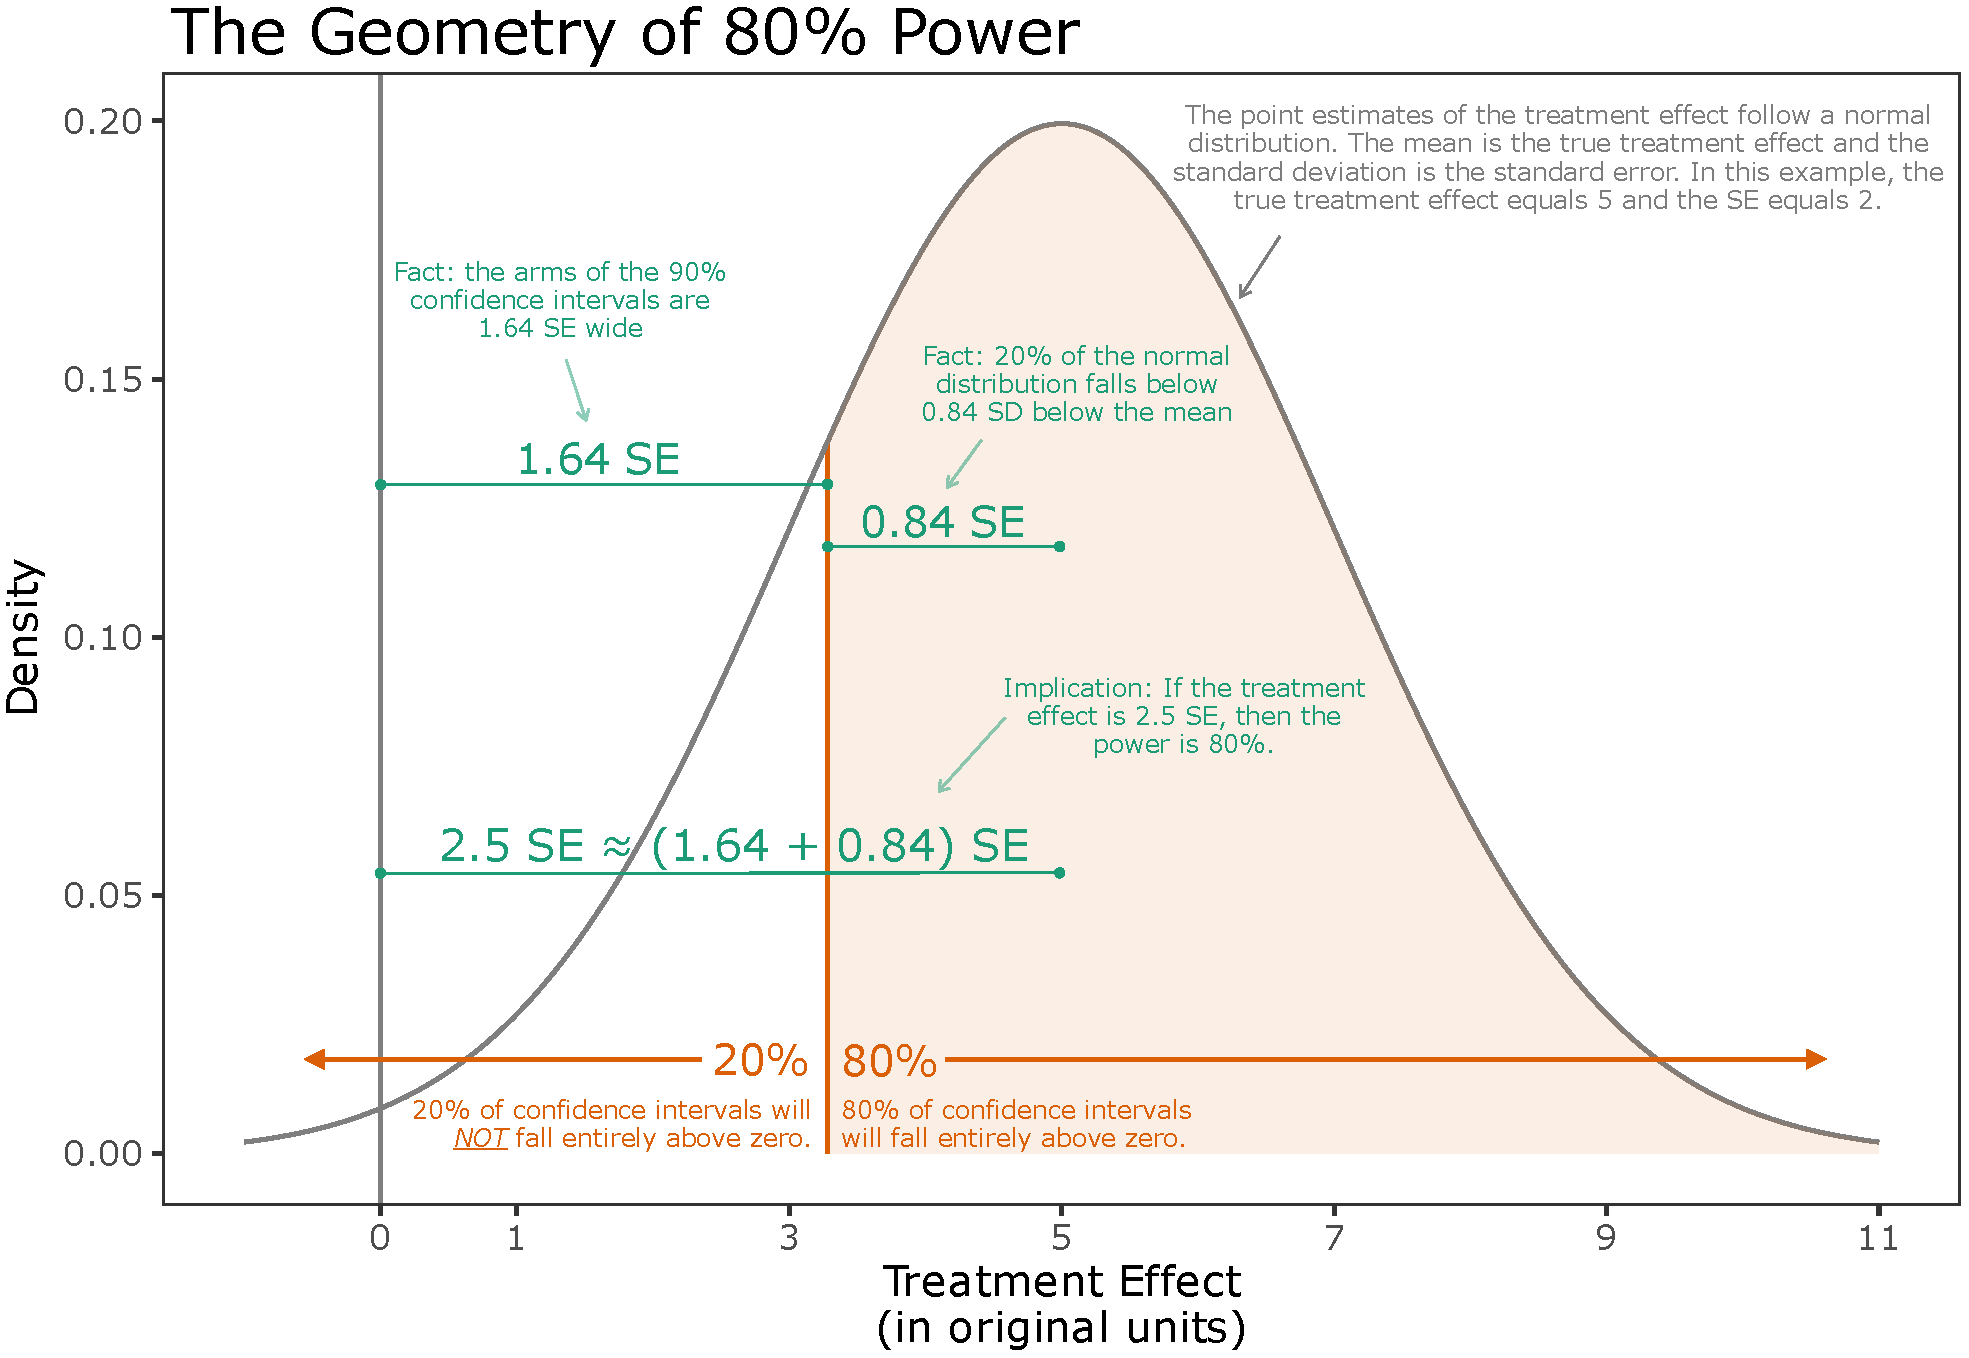
\includegraphics[width=\linewidth]{geometry.pdf}
    \caption{This figure shows why experiments have 80\% power to detect effects that are 2.5 standard errors. The arms of the 90\% confidence interval are 1.64 standard errors wide, so the power of the study is the percent of the sampling distribution that is larger than 1.64 standard errors. If we plug 0.80 into the inverse of the standard normal CDF, we obtain 0.84. To position 80\% of the sampling distribution above 1.64 standard errors, the sampling distribution must be centered (1.64~+~0.84) = 2.48 standard errors above zero, which we can safely treat as 2.5. The figure depicts the one-sided test. A two-sided test replaces 1.64 with 1.96, which shifts the 2.48 factor to 2.80.}
    \label{fig:intuition}
\end{figure}

\section*{Example: Evaluating Power for a Fixed Sample Size}

In many research contexts, we do not choose the sample size.
For example, it is common to include survey experiments on modules of the Cooperative Election Study (CES), which include 1,000 respondents.
Or we might have the opportunity to include an experiment on a survey designed for another purpose.
Or we might want to conduct an experiment on the entire population of interest.
In this context, we simply need to know whether our already-determined sample size provides sufficient statistical power.
Rules~\ref{rule:sd-to-se},~\ref{rule:adjustment}, and~\ref{rule:se-to-mde} allow us to work in this context.

As an example, imagine we are planning to replicate Ahler and Sood's (\citeyear{Ahler2018}) finding that correcting respondents' misperceptions of their out-party reduces affective polarization.
If we are planning to replicate the finding on a CES module, then we will have 1,000 respondents total or 500 respondents in each of the treatment and control conditions.
Do 1,000 respondents provide sufficient statistical power?

In the original experiment, the treatment has two steps.
First, Ahler and Sood (1) ask Republicans to report their perceptions of the percent of Democrats with certain demographic attributes and (2) ask Democrats to report their perceptions of the percent of Republicans with certain demographic attributes.
Second, after asking respondents to report their perceptions of the out-party, Ahler and Sood provide respondents with the correct information.
Compared to a control group that was neither asked their perceptions beforehand nor given the correct information, the treatment group evaluated supporters of the out-party more favorably on a 101-point feeling thermometer scale.
They estimate a treatment effect of 6.4 points on the 101-point scale with a 95\% confidence interval of [3, 10].
As part of a much larger study, \citet{Broockman2022} closely replicate Ahler and Sood's result. My re-analysis of their data\footnote{The replication data and code for this article are available in the \emph{Political Analysis} Dataverse at \url{https://doi.org/10.7910/DVN/EMLFBT} (\citealt{Rainey2026data}).} gives an estimated treatment effect of 3.9 with a 90\% confidence interval of [1.1, 6.6].\footnote{
  \citet{Broockman2022} report a slightly different analysis in the main text of their paper.
  Most notably, they use the difference between evaluations of the ``people who are'' the in-party and ``people who are'' the out-party.
  Using their replication data \citep{BKW2022data}, I run an analysis that treats evaluations of ``people who are'' the out-party as the outcome (instead of the difference).
  This latter, alternative analysis is similar to Ahler and Sood's approach, so I focus on it here.}
In both cases, the 90\% confidence interval includes only positive effects, so we reject the null hypothesis that the treatment effect is less than or equal to zero and conclude that the treatment has the hypothesized positive effect on the feeling thermometer toward supporters of the out-party.

How could we use features of a reference population along with Rules~\ref{rule:sd-to-se},~\ref{rule:adjustment}, and~\ref{rule:se-to-mde} to evaluate our study?
Our goal is to use Rule~\ref{rule:sd-to-se} to predict the standard error, use Rule~\ref{rule:adjustment} to account for any control variables we plan to use, and use Rule~\ref{rule:se-to-mde} to find the minimum detectable effect with 80\% and 95\% power.
If that minimum detectable effect is sufficiently small, then we will say that our study has adequate statistical power.

\subsection*{Without Control Variables: Rules~\ref{rule:sd-to-se} and~\ref{rule:se-to-mde}}

Using Rule~\ref{rule:sd-to-se}, the standard error will be about $\frac{2 \cdot \widetilde{SD(Y)}}{\sqrt{2 \cdot n}}$.
In this context, $n = 500$ because we have two experimental conditions and $N = 1{,}000$ in a CES module.
However, we must plug a suitable value for $\widetilde{SD(Y)}$ into the equation. For this application, and many others, we can think of $\widetilde{SD(Y)}$ as the standard deviation of the outcome in the control group (or treatment group if that is easier).

In practice, we can look to standard deviations in reference populations ``like'' our experimental sample.\footnote{In a pinch, we can imagine the responses are spread roughly evenly across the scale. For this even spread, the standard deviation is about the range (max $-$ min) divided by $\sqrt{12} \approx 3.5$ (because a uniform distribution on $[0, 1]$ has a standard deviation of $1/\sqrt{12}$). For a feeling thermometer, we have $100/\sqrt{12} \approx 28.9$. However, this rough rule should be used only as a first approximation, if used at all. \citet{Hozo2005} and \citet{Wan2014} develop related range-based approximations that recover a standard deviation from a reported median, range, and sample size.}
For example, the American National Election Studies (ANES) asked a similar question in 2020.
The ANES version asks respondents to report their feelings toward the Democratic [Republican] party, while Ahler and Sood ask respondents to report their feelings toward \emph{supporters of} the Democratic [Republican] party.
The standard deviation of the responses to the similar ANES question is 20.8 \citep{ANES2026}.

Using Rule~\ref{rule:sd-to-se}, the standard error in our replication will be about $\frac{2 \cdot \widetilde{SD(Y)}}{\sqrt{2 \cdot n}} = \frac{2 \cdot 20.8}{\sqrt{2 \cdot 500}} = 1.32$.
Using Rule~\ref{rule:se-to-mde}, a standard error of 1.32 means that we will have 80\% power to detect a treatment effect of $2.5 \cdot SE = 2.5 \cdot 1.32 = 3.30$ points on the 101-point scale and have 95\% power to detect a treatment effect of $3.3 \cdot SE = 3.3 \cdot 1.32 = 4.36$ points (a two-sided test would use 2.8 and 3.6, giving 3.70 and 4.75 points).
As substantive experts, if we determine that these effects are acceptable (e.g., they correspond to the smallest substantively meaningful effect), then the experiment has adequate statistical power.


\subsection*{With Control Variables: Rules~\ref{rule:sd-to-se},~\ref{rule:adjustment}, and~\ref{rule:se-to-mde}}

To shrink the standard error (and the minimum detectable effect along with it), we can consider the adjustment strategy of \citet{Broockman2022}.
They control for a seven-point party identification scale and partisan strength.
Rule~\ref{rule:adjustment} states that regression adjustment will shrink the unadjusted standard error by about $\left\lbrack 1 - \sqrt{ 1 - \widetilde{R^{2}} } \right\rbrack \cdot 100\%$, but we need to choose a suitable value of $\widetilde{R^{2}}$ to plug into the equation.

In the 2020 ANES, the seven-point party identification scale and partisan strength scale have an $R^{2}$ of 5\% for the similar feeling thermometer toward the out-party (rather than ``supporters of'' the out-party).
For $\widetilde{R^{2}} = 5\%$, this adjustment strategy will shrink the standard error by about $\left\lbrack 1 - \sqrt{ 1 - \widetilde{R^{2}} } \right\rbrack = \left\lbrack 1 - \sqrt{1 - 0.05} \right\rbrack = 2.5\%$.
This strategy is perhaps worth pursuing, but will not change the standard error dramatically.\footnote{It seems reasonable, too, that these two variables will explain less variation in feelings toward partisans than toward the parties themselves, so this $R^{2}$ of 5\% might be too high. Indeed, my re-analysis of Broockman, Kalla, and Westwood's data shows that these two control variables produce an $R^{2}$ of 1.0\% in the control group and 1.8\% in the treatment group. An $R^{2}$ of 1.4\% (which is the average of the two) will shrink the standard error by about 0.7\%. This difference is negligible compared to a strategy without control variables.}

Adding the adjustment to our calculation, our standard error will be about $\frac{2 \cdot \widetilde{SD(Y)}\cdot \sqrt{1 - \widetilde{R^{2}}}}{\sqrt{2 \cdot n}} = \frac{2 \cdot 20.8 \cdot \sqrt{1 - 0.05}}{\sqrt{2 \cdot 500}} = 1.28$.
Using Rule~\ref{rule:se-to-mde}, a standard error of 1.28 means that we will have 80\% power to detect a treatment effect of $2.5 \cdot SE = 2.5 \cdot 1.28 = 3.20$ points on the 101-point scale and have 95\% power to detect a treatment effect of $3.3 \cdot SE = 3.3 \cdot 1.28 = 4.22$ points.
The minimum detectable effects using Broockman, Kalla, and Westwood's adjustment strategy are practically the same as those without any adjustment.

However, \citet{Clifford2021} offer a potentially promising approach here.
They suggest measuring the outcome both before and after the treatment and then controlling for the pre-treatment measure.
This pre-treatment measure should be \emph{strongly} related to the post-treatment outcome.
As an initial guess, we might let $\widetilde{R^{2}} = 40\%$, which falls at the low end of the range of $R^{2}$ (about 37\% to 81\%) that \citet[1059]{Clifford2021} observe across their five pre-post studies.
With $\widetilde{R^{2}} = 40\%$, the standard error will be about $\frac{2 \cdot 20.8 \cdot \sqrt{1 - 0.40}}{\sqrt{2 \cdot 500}} = 1.02$.
For a standard error of 1.02, we will have 80\% power to detect a treatment effect of $2.5 \cdot SE = 2.5 \cdot 1.02 = 2.55$ points on the 101-point scale and 95\% power to detect a treatment effect of $3.3 \cdot SE = 3.3 \cdot 1.02 = 3.37$ points.\footnote{
  We should do additional work to confirm this initial guess.
  In a pilot study, \citet{Cutler2024} test a strategy of measuring the out-party feeling thermometer before and after the treatment.
  They find that the pre-treatment measure has an $R^{2}$ of about 76\%.
  This suggests that the pre-post strategy will shrink the standard error by about 51\%.}
This adjustment strategy might make a difference in whether we consider our 1,000-respondent study adequately powered.

\section*{Rule~\ref{rule:sd-to-sample-size}: From the SD to the Sample Size}

Rule~\ref{rule:se-to-mde} is helpful---it gives us the minimum detectable effect for a given study.
But it does not produce the sample size that we need to obtain 80\% or 95\% power.
To find the sample size that produces our desired minimum detectable effect (usually the smallest substantively meaningful effect), we can combine Rules~\ref{rule:sd-to-se},~\ref{rule:adjustment}, and~\ref{rule:se-to-mde}.
Suppose we want our experiment to have 80\% power to detect the effect $\widetilde{\tau}$.
Then we need $\widetilde{\tau} = 2.5 \cdot SE = 2.5 \cdot \frac{2 \cdot \widetilde{SD(Y)}}{\sqrt{2 \cdot n}}$.
Solving for $n$, we find that we will need $2 \cdot \left( \frac{2.5 \cdot \widetilde{SD(Y)}}{\widetilde{\tau}} \right)^{2}$ respondents per condition (rounded up) to obtain 80\% power.
If we are adjusting for control variables, we need $2 \cdot \left( \frac{2.5 \cdot \widetilde{SD(Y)} \cdot \sqrt{1 - \widetilde{R^{2}}}}{\widetilde{\tau}} \right)^{2}$ respondents per condition for 80\% power. For 95\% power to detect the effect $\widetilde{\tau}$, the factor changes from 2.5 to 3.3, and we need $2 \cdot \left( \frac{3.3 \cdot \widetilde{SD(Y)}}{\widetilde{\tau}} \right)^{2}$ or $2 \cdot \left( \frac{3.3 \cdot \widetilde{SD(Y)} \cdot \sqrt{1 - \widetilde{R^2}}}{\widetilde{\tau}} \right)^{2}$ respondents per condition, respectively.\footnote{
  This leads to another useful rule of thumb, though this one is rough.
  Suppose that we are interested in effects that are 10\% of a standard deviation.
  (\citet{Lovakov2021} find that about one in five effects in social psychology is smaller than 11\% of a standard deviation.)
  Then the term $\left( \frac{\widetilde{SD(Y)}}{\widetilde{\tau}} \right)^{2}$ equals 100, so we can simply multiply the factors $2 \cdot {2.5}^{2} = 12.5$ and $2 \cdot {3.3}^{2} = 21.8$ by 100 to find the required sample sizes of 1,250 and 2,180 per condition to detect these ``small'' effects with 80\% and 95\% power.
  For a two-sided test, the factors are $2 \cdot {2.8}^{2} = 15.7$ and $2 \cdot {3.6}^{2} = 25.9$, giving 1,570 and 2,590 respondents per condition.
  }

\begin{restatable}[SD to Sample Size]{rule0}{rulesdtosamplesize}
\label{rule:sd-to-sample-size}
We can use features of a reference population to compute the sample size we will need in a planned study.
For 80\% power to detect the treatment effect $\widetilde{\tau}$, the sample size per condition will need to be about $2 \cdot \left( \frac{2.5 \cdot \widetilde{SD(Y)}}{\widetilde{\tau}} \right)^{2}$ (or $2 \cdot \left( \frac{2.5 \cdot \widetilde{SD(Y)} \cdot \sqrt{1 - \widetilde{R^{2}}}}{\widetilde{\tau}} \right)^{2}$ if including control variables), where $\widetilde{SD(Y)}$ is the standard deviation of the outcome in a reference population and $\widetilde{R^2}$ is the $R^2$ of a regression of the outcome on the control variables in a reference population.
For 95\% power, the factor changes from 2.5 to 3.3.
\end{restatable}

{\noindent \footnotesize\textit{Note: For a two-sided test, the factors are 2.8 and 3.6. See Table~\ref{tbl:factors}.}}

\section*{Example: Finding the Sample Size}

In the examples above, we imagined a research context in which the sample size was not under our control.
But in many contexts, we can control (or must choose) the sample size.
Continuing our example of Ahler and Sood's (\citeyear{Ahler2018}) experiment from above, we can use features of a reference population to predict the required sample size.
For simplicity, suppose that we would like 95\% power to detect a treatment effect of 3 points on the 101-point scale.\footnote{A 3-point effect on the 101-point scale is the lower bound of Ahler and Sood's 95\% confidence interval.}

Above, we use the ANES to motivate setting $\widetilde{SD(Y)}$ to 20.8 and $\widetilde{R^{2}}$ to 5\%.
Rule~\ref{rule:sd-to-sample-size} tells us that, without control variables, we will need about $2 \cdot \left( \frac{3.3 \cdot \widetilde{SD(Y)}}{\widetilde{\tau}} \right)^{2} = 2 \cdot \left( \frac{3.3 \cdot 20.8}{3} \right)^{2} = 1{,}047$ respondents per condition for 95\% power.
With control variables that predict the outcome with an $R^2$ of 5\%, this becomes ${2 \cdot \left( \frac{3.3 \cdot \widetilde{SD(Y)} \cdot \sqrt{1 - \widetilde{R^{2}}}}{\widetilde{\tau}} \right)}^{2} = 2 \cdot \left( \frac{3.3 \cdot 20.8 \cdot \sqrt{1 - 0.05}}{3} \right)^{2} = 995$ respondents per condition.

A researcher who prefers a two-sided test (a 95\% confidence interval) would use the factor 3.6 in place of 3.3 (Table~\ref{tbl:factors}).
Without control variables, this requires $2 \cdot \left( \frac{3.6 \cdot \widetilde{SD(Y)}}{\widetilde{\tau}} \right)^{2} = 2 \cdot \left( \frac{3.6 \cdot 20.8}{3} \right)^{2} = 1{,}247$ respondents per condition.
This is about 19\% more than the 1,047 the one-sided test requires.

\section*{Rule~\ref{rule:80-to-95}: From 80\% Power to 95\% Power}

In thinking about the tradeoff between 80\% and 95\% power, it can be helpful to have a rule connecting sample size requirements.
The square root law tells us that standard errors depend on the sample size by a factor of $\frac{1}{\sqrt{n}}$, so the ratio of two standard errors ${SE}_{\widehat{\tau}}^{A}$ and ${SE}_{\widehat{\tau}}^{B}$ with sample sizes $n^{A}$ and $n^{B}$ per condition, respectively, is $\frac{SE_{\widehat{\tau}}^{A}}{SE_{\widehat{\tau}}^{B}} = \sqrt{\frac{n^{B}}{n^{A}}}$.
For an assumed treatment effect $\widetilde{\tau}$, the standard errors that yield 80\% power (design $A$) and 95\% power (design $B$) are given by $\frac{\widetilde{\tau}}{2.5}$
and $\frac{\widetilde{\tau}}{3.3}$, respectively.
Then we have $\frac{SE_{\widehat{\tau}}^{A}}{SE_{\widehat{\tau}}^{B}} = \frac{\frac{\widetilde{\tau}}{2.5}}{\frac{\widetilde{\tau}}{3.3}} = \frac{3.3}{2.5} = \sqrt{\frac{n^{B}}{n^{A}}}$.
Then we can see that $\frac{n^{B}}{n^{A}} = \left( \frac{3.3}{2.5} \right)^{2} = 1.74$. This means that to increase the power from 80\% to 95\%, we need to increase our sample size by about 74\%.
With less rounding error, this becomes 75\%.

For a two-sided test, the standard errors that yield 80\% and 95\% power are $\frac{\widetilde{\tau}}{2.8}$ and $\frac{\widetilde{\tau}}{3.6}$, so $\frac{n^{B}}{n^{A}} = \left( \frac{3.6}{2.8} \right)^{2} \approx 1.65$, an increase of about 65\%.
With less rounding error, this becomes 66\%.

\begin{restatable}[80\% to 95\% Power]{rule0}{ruleconvert}
\label{rule:80-to-95}
Increasing the sample size by about 75\% will increase the power from 80\% to about 95\%.
\end{restatable}

{\noindent \footnotesize\textit{Note: For a two-sided test, increasing the sample size by about 66\% will increase the power from 80\% to about 95\%.}}

\noindent The rules also extend to hypotheses about interactions, with two minor modifications that I describe in~Appendix~2.

\section*{How to Use the Rules}

Table~\ref{tbl:how} shows how we can use the rules to establish that a planned experiment is well-powered. Broadly, there are three strategies, or ways to arrange our thinking:

\begin{enumerate}
\item For a given sample size and statistical power, show that the minimum detectable effect corresponds to a ``small'' effect, either the smallest substantively meaningful effect or the smallest plausible effect given the available evidence.
\item For a given sample size and effect of interest, show that the statistical power of the experiment is greater than a chosen threshold (e.g., 80\% or 95\%).
\item For a given statistical power and effect of interest, show that the sample size meets (or exceeds) the required sample size.
\end{enumerate}

\noindent However, we should not draw strong distinctions between these strategies---the strategies differ only in the order in which the sample size, effect of interest, and statistical power are chosen.
In the end, it simply matters that the three components combine to form a well-powered experiment.

To make each of these arguments, we need features of a reference population: studies that measure our outcome (and perhaps control variables) on a similar population.
We can use the standard deviation and $R^2$ in this reference population to predict the standard deviation and $R^2$ in our planned study.
Table~\ref{tbl:how} summarizes the rules.
For each goal, it lists the information needed, the rules to apply, and the equations those rules produce (written for 80\% power).

\begin{table}[ht]
\centering
\caption{This table shows how we can use the rules to answer questions about the experiment using features of a reference population. The ``Equations'' column gives one equation per rule in the indicated sequence. The equations are written for the one-sided test at 80\% power. For 95\% power, replace 2.5 with 3.3. For a two-sided test, replace 2.5 and 3.3 with 2.8 and 3.6 and replace 1.64 with 1.96 in the power equations (see Rules~\ref{rule:power-z} and~\ref{rule:se-to-mde} and Table~\ref{tbl:factors}).}\label{tbl:how}
\setlength{\extrarowheight}{8pt}
\renewcommand{\arraystretch}{1.4}
\setlength{\tabcolsep}{10pt}
\scriptsize
\renewcommand\tabularxcolumn[1]{>{\centering\arraybackslash}m{#1}}
\noindent\makebox[\textwidth][c]{%
\begin{tabularx}{\dimexpr\textwidth+0.667in\relax}{>{\hsize=0.75\hsize\linewidth=\hsize}X>{\centering\arraybackslash}m{2cm}>{\centering\arraybackslash}m{2.4cm}>{\centering\arraybackslash}m{1.4cm}>{\hsize=1.25\hsize\linewidth=\hsize}X}
\toprule
\headrow {\footnotesize\textbf{Goal}} & {\footnotesize\textbf{Estimation Strategy}} & {\footnotesize\textbf{Required Information}} & {\footnotesize\textbf{Rule Sequence}} & {\footnotesize\textbf{Equations}} \\
\midrule
I know my sample size and the statistical power I want. What is my minimum detectable effect?
 & no control variables
 & $SD(Y)$ in reference population
 & Rule~\ref{rule:sd-to-se}\par$\downarrow$\par Rule~\ref{rule:se-to-mde}
 & $SE = \dfrac{2 \cdot \widetilde{SD(Y)}}{\sqrt{2n}}$ \par\medskip
   $MDE_{80\%} = 2.5 \cdot SE$ \\[8pt]
\cmidrule(lr){2-5}
 & control variables
 & $SD(Y)$ and $R^2$ of control variables in reference population
 & Rule~\ref{rule:sd-to-se}\par$\downarrow$\par Rule~\ref{rule:adjustment}\par$\downarrow$\par Rule~\ref{rule:se-to-mde}
 & $SE = \dfrac{2 \cdot \widetilde{SD(Y)}}{\sqrt{2n}}$ \par\medskip
   $SE^{adj} = SE \cdot \sqrt{1 - \widetilde{R^{2}}}$ \par\medskip
   $MDE_{80\%} = 2.5 \cdot SE^{adj}$ \\[8pt]
\midrule
I know my sample size and the effect of interest. What is my statistical power?
 & no control variables
 & $SD(Y)$ in reference population
 & Rule~\ref{rule:sd-to-se}\par$\downarrow$\par Rule~\ref{rule:power-z}
 & $SE = \dfrac{2 \cdot \widetilde{SD(Y)}}{\sqrt{2n}}$ \par\medskip
   $Power = 1 - \Phi_{std}\!\left( 1.64 - \dfrac{\widetilde{\tau}}{SE} \right)$ \\[8pt]
\cmidrule(lr){2-5}
 & control variables
 & $SD(Y)$ and $R^2$ of control variables in reference population
 & Rule~\ref{rule:sd-to-se}\par$\downarrow$\par Rule~\ref{rule:adjustment}\par$\downarrow$\par Rule~\ref{rule:power-z}
 & $SE = \dfrac{2 \cdot \widetilde{SD(Y)}}{\sqrt{2n}}$ \par\medskip
   $SE^{adj} = SE \cdot \sqrt{1 - \widetilde{R^{2}}}$ \par\medskip
   $Power = 1 - \Phi_{std}\!\left( 1.64 - \dfrac{\widetilde{\tau}}{SE^{adj}} \right)$ \\[8pt]
\midrule
I know the statistical power I want and the effect of interest. What sample size do I need?
 & no control variables
 & $SD(Y)$ in reference population
 & Rule~\ref{rule:sd-to-sample-size}
 & $n_{80\%} = 2 \cdot \left( \dfrac{2.5 \cdot \widetilde{SD(Y)}}{\widetilde{\tau}} \right)^{\!2}$ \\[8pt]
\cmidrule(lr){2-5}
 & control variables
 & $SD(Y)$ and $R^2$ of control variables in reference population
 & Rule~\ref{rule:sd-to-sample-size}
 & $n_{80\%} = 2 \cdot \left( \dfrac{2.5 \cdot \widetilde{SD(Y)} \cdot \sqrt{1 - \widetilde{R^{2}}}}{\widetilde{\tau}} \right)^{\!2}$ \\[8pt]
\bottomrule
\end{tabularx}}
\end{table}

\section*{Related Work}

\citet{Cohen1988} provides the foundational introduction to power analysis, and \citet{Cohen1990} offers an engaging personal and historical perspective.
\citet[ch.~9]{DeGroot2010} and \citet[ch.~8]{Casella2002} provide a thorough technical discussion.
\citet{Greenland2016} offer an accessible and intuitive discussion organized around potential \textit{mis}understandings of the concepts.
\citet{Bloom1995} offers a particularly practical and intuitive approach using the minimum detectable effect.
\citet{Cohen1992}, \citet{Lenth2001}, and \citet{Meyvis2017} also offer practical guides.
\citet{Rainey2014}, \citet{McCaskey2015}, and \citet[see esp.~261--263]{Lakens2018} discuss the smallest effects of substantive interest, and \citet{Lovakov2021} offer empirical rules for effect sizes derived from social psychology.
\citet{Lakens2022} offers a broader perspective on sample size justification beyond statistical power.
\citet{Blair2019} and \citet{Blair2023} offer a useful conceptual framework and software for comprehensive evaluation of research designs.
In a companion paper, I offer advice on using existing studies and pilot data to automate power analysis \citep{Rainey2024pilot}.

Several well-known rules of thumb relate closely to the ones I offer here.
Rule~\ref{rule:se-to-mde} is essentially \citeauthor{Bloom1995}'s (\citeyear{Bloom1995}) minimum detectable effect, named explicitly in the rule.
Rule~\ref{rule:sd-to-sample-size} is the one-sided counterpart of \citeauthor{Lehr1992}'s (\citeyear{Lehr1992}) rule of $n \approx 16/\Delta^2$ per group (where $\Delta = \widetilde{\tau}/\widetilde{SD(Y)}$), with coefficient 12.5 in place of 16.
Lehr's own table of coefficients gives 12.5 for two-tailed $\alpha = 0.10$, which matches my one-sided $\alpha = 0.05$ convention.
Under the two-sided $\alpha = 0.05$ convention, the coefficient becomes $2 \cdot {2.8}^{2} \approx 15.7$, essentially Lehr's (\citeyear{Lehr1992}) 16.
Both rules require a guess at the effect size, and \citet[25--26]{Cohen1988} supplies the familiar small, medium, and large benchmarks of $\Delta = 0.2$, $0.5$, and $0.8$ that many researchers use as defaults.
\citet{Lovakov2021} update these benchmarks with empirical effect-size distributions from social psychology, where about one in five effects is smaller than $\Delta = 0.11$.
Andrew Gelman's well-known ``you need 16 times the sample size to estimate an interaction than to estimate a main effect'' follows from Rule~\ref{rule:sd-to-sample-size}, modified for interactions in~Appendix~2, under the assumption that the interaction is half the size of the main effect.
Finally, \citeauthor{Simonsohn2015}'s (\citeyear{Simonsohn2015}) $d_{33}$ and 2.5$\times$ replication rule, derived in~Appendix~3, both follow from Rule~\ref{rule:se-to-mde} (the latter approximately).


\section*{Conclusion}

To address the problem of low power in political science research \citep{ArelBundock2022} and increasing requirements that articles, registered reports, and grant applications include a power analysis, I offer several useful rules that help political scientists reason about statistical power.
For balanced, between-subjects designs to estimate treatment effects and/or interactions, these rules are sufficient to justify a sample size.
These rules are not meant to cover every experiment.
Appendix~1 and~Appendix~2 extend the rules, including to power levels other than 80\% or 95\%, unbalanced assignment, clustered assignment, blocked random assignment, and interactions.
More complicated designs require simulation or specialized software, but even then the rules can provide a useful first approximation and help us avoid big errors.

Perhaps most importantly, these rules help develop intuitions about statistical power.
For example, these rules can help us quickly appreciate the tradeoffs between spreading survey respondents across eight conditions rather than four, or between using fewer respondents through a more expensive provider or more respondents through a less expensive provider.

In this paper, I focus mostly on the choice of sample size, but there are more (and sometimes better) ways to increase statistical power.
Keep Rule~\ref{rule:se-to-mde} top of mind: we must get the ratio of the assumed treatment effect and the standard error above 2.5 and ideally above 3.3 (2.8 and 3.6 for a two-sided test).
The task is clear---we need a treatment with oomph to make the numerator large and strategies like regression adjustment, precise measurement instruments, attentive respondents, and large samples to make the standard error small.\footnote{
  Although \citet{Kane2025} frames his essay as a guide to anticipating and investigating nonsignificant results, he describes several strategies to increase treatment effects and decrease the standard error.
  }
I hope these rules help us think carefully about these efforts.


\paragraph{Acknowledgments}
I used Claude models from Anthropic in 2025--2026 agentically (via Claude Code) for project and file management (e.g., repository organization, build automation, and version control), code development (e.g., organizing the replication materials at \url{https://doi.org/10.7910/DVN/EMLFBT}), and error-checking. All writing, analysis, and conclusions are my own, and I am solely responsible for the article's content.

\paragraph{Competing Interests}
None.

\paragraph{Data Availability Statement}
Replication code and data for this article are available in the \emph{Political Analysis} Dataverse at \url{https://doi.org/10.7910/DVN/EMLFBT} (\citealt{Rainey2026data}).

\printbibliography

%%% end body
\end{document}
